
%\chapter{Experimental setup}
\label{sec:setup:phys-signals}

The clinical symptoms of migraine are widely accepted to be related to
the autonomic nervous system (ANS) \cite{melek2007autonomic,
sanya2005impairment, barbanti2013dopaminergic, gass2013autonomic,
becker2013premonitory, hassinger1999cardiovascular}. In contrast to
the somatic nervous system, which provides voluntary control of the
body, the ANS is the part of the peripheral nervous system that
controls visceral functions, acting largely below the level of
consciousness. Consequently, the ANS controls vital signs including
heart rate, digestion, respiration rate, vomiting and swallowing.


In the migraine disease, the involvement of the ANS is materialized in
a dysfunction in the regulation of the circulatory system and the
autonomic balance. As described in \cite{mendes2009assessing}, there
are several biometric variables that allow to assess changes in ANS
activity. Some of them and others have already been studied in
migraineurs: electrocardiogram (ECG) \cite{melek2007autonomic,
aygun2003electrocardiographic}, heart rate \cite{pmid23853566,
pmid19925627}, skin temperature \cite{zaproudina2013acral,
ordas2013increase}, blood pressure \cite{pietrini2005hypertension,
pmid19925627} and electroencephalogram
(EEG) \cite{bjork2011initiates}. The system used was able to register
all these signals and two more variables: oxygen saturation and
sweating, monitored as electrodermal activity. Both, oxygen saturation
and sweating, are related to the ANS too.

The main characteristics of the above-mentioned physiological signals
are described below.

\subsection{Electrocardiogram}
\label{subsec:setup:phys-signals:ecg}

An electrocardiogram (ECG) describes the electrical impulses that
travel through the heart. It provides information about the rate,
rhythm, and morphology of the heart.

\begin{figure}[!ht]
\centering
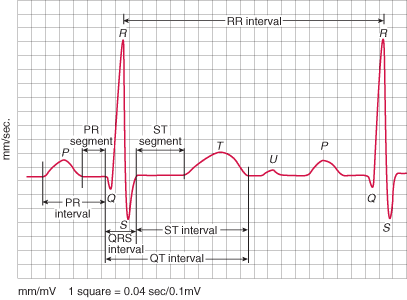
\includegraphics[width=0.8\textwidth]{images/ECGwave.png}
\caption{ECG wave}
\label{fig:ecg}
\end{figure}


A typical ECG wave of a normal heartbeat is described
in \cite{wang2008analysis}. It consists of a P wave, a QRS complex,
and a T wave as shown in \figref{ecg}. The first wave reflects the
sequential depolarization of the right and left atria. It usually has
positive polarity, and its duration is less than 120 milliseconds. The
spectral characteristic of a normal P wave is usually considered to be
low frequency, below 10–15 Hz. The QRS complex corresponds to the
depolarization of the right and left ventricles. It lasts for about
70–110 milliseconds in a normal heartbeat, and has the largest
amplitude of the ECG waveforms. Due to its steep slopes, the frequency
content of the QRS complex is considerably higher than that of the
other ECG waves, and is mostly concentrated in the interval of 10–40
Hz. The T wave reflects ventricular repolarization and extends about
300 milliseconds after the QRS complex. The position of the T wave is
strongly dependent on heart rate, becoming narrower and closer to the
QRS complex at rapid rates.


Normally, ECG is recorded by attaching a set of electrodes on the
chest, neck, arms, and legs.


\subsection{Pulse oximetry and plesthymographic curve}
\label{subsec:setup:phys-signals:ppg}


The pulse oximetry offers real-time assessment of oxygenation status
on a moment-to-moment basis. The foundation for pulse oximetry is the
spectral analysis: the detection and quantitation of oxygenated and
deoxygenated (or reduced) hemoglobin by their unique light absorption
characteristics \cite{sinex1999pulse, bagha2011real}.

\begin{figure}[!ht]
\centering
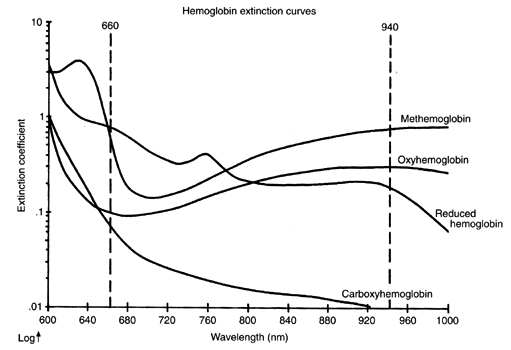
\includegraphics[width=0.9\textwidth]{images/hemoglobin.png}
\caption{Absorption of the red and the infrared lights by oxygenated and reduced hemoglobin}
\label{fig:hemoglobin}
\end{figure}



Two LEDs in the pulse oximeter emit light of specific wavelength
through a cutaneous vascular bed. A photodiode detector at the far
side measures the intensity of transmitted light at each wavelength,
from which oxygen saturation (SpO2) can be
derived \cite{bagha2011real}. \figref{hemoglobin} shows how oxygenated
hemoglobin absorbs more infrared light (910 nm) and allows more red
light (660 nm) to pass through, whereas reduced hemoglobin absorbs
more red light and allows more infrared light to pass through.


In the process of determining SpO2, the pulse oximeter functions as a
photoelectric plethysmograph. In this role, it measures changes in the
light absorption of the vascular bed. The resulting photoplesthymogram
(PPG) comprises a pulsatile physiological waveform attributed to
cardiac synchronous changes in the blood volume with each
heartbeat \cite{allen2007photoplethysmography}. This signal, shown
in \figref{bloodpressure}, is superimposed on a slowly varying
baseline with various lower frequency components attributed to
respiration, sympathetic nervous system activity and
thermoregulation. \figref{PPGnatvars} shows a complete picture of the
PPG waveform.

\begin{figure}[!ht]
\centering
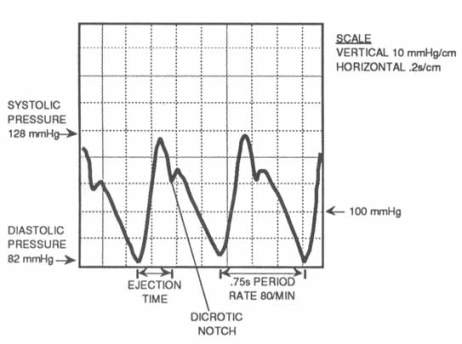
\includegraphics[width=0.8\textwidth]{images/BloodPressureWaveform.jpg}
\caption{Cardiac synchronous changes in the blood volume}
\label{fig:bloodpressure}
\end{figure}


\begin{figure}[!ht]
\centering
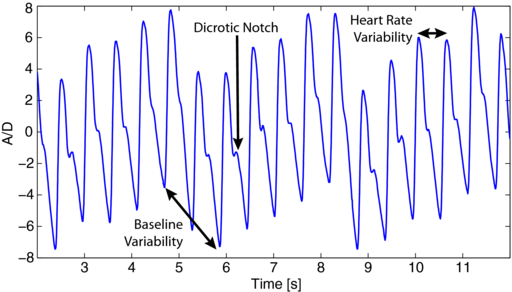
\includegraphics[width=0.8\textwidth]{images/PPGnaturalVariations.jpg}
\caption{PPG waveform}
\label{fig:PPGnatvars}
\end{figure}



Pulse oximetry is usually measured on skin surfaces with high
capillarity, such as that of the digits or the ear lobe.


\subsection{Heart rate}
\label{subsec:setup:phys-signals:hr}

The heart rate (HR) refers to the number of beats that the heart
performs in a time interval. It is usually expressed in beats per
minute.

ECG and PPG can be sources of instantaneous HR information, since both
signals present synchronous changes with each cardiac beat. In the
first case, HR is calculated through R-R intervals. In the PPG curve,
we can consider as the reference point the one in which the amplitude
of the waveform is maximum. Then, HR can be obtained from the time
interval existing between two consecutive reference
points. \figref{HRcalculus} shows these ECG and PPG parameters related
to the HR calculus.


\begin{figure}[!ht]
\centering
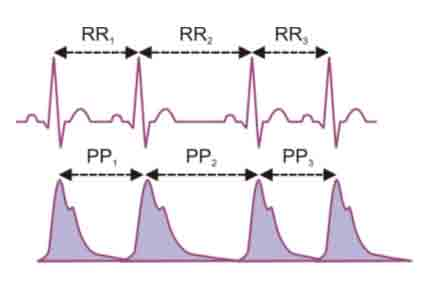
\includegraphics[width=0.6\textwidth]{images/PPGandECG.jpg}
\caption{ECG and PPG parameters related to the HR calculus}
\label{fig:HRcalculus}
\end{figure}


% \subsubsection{Blood pressure and pulse transit time}

% The pressure pulse generated by ventricular ejection is propagated through the arterial tree. The propagation velocity is determined by the elastic and geometric properties of the arterial wall and the blood density. Blood pressure (BP) is a commonly used parameter which carries important information about the status of the cardiovascular system.

% The measurement of pulse wave velocity (PWV), which is inversely related to arterial wall distensibility, offers a simple and potentially useful approach to measure the BP. Pulse transit time (PTT), defined as the time interval between the peak time of the R wave (ECG signal) and the time when pulse waveforms reach their maximum value (PPG signal), is one of the most common proposals for the non-invasive PWV estimation. Figure \ref{fig:PTTdet} shows this relationship among ECG, PPG and PTT.

% The explanation of how PTT and BP relate to each other is described in detail in \cite{choi2004evaluation, wong2005effects}.

% Since the PTT signal represents the time needed by a pulse wave to exit the heart and reach the place where PPG is measured, the larger the distance between that place and the heart, the lesser impact measurement error will have on the PTT determination. For this reason the pulse wave is usually detected at the fingertip \cite{hey2009continuous}.In this project, we will make use of the direct correlation between the PPG curve, the ECG curve and the BP estimation through PTT. However, we will avoid to work with absolute values of BP that would require the validation of the measure for every patient.

% \begin{figure}[!ht]
% \centering
% 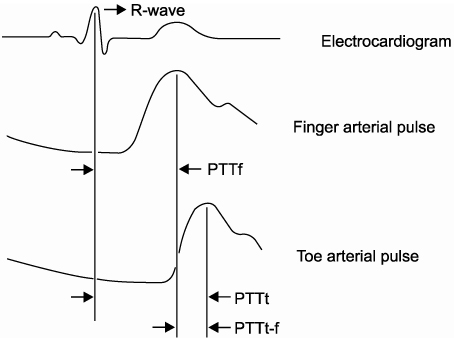
\includegraphics[width=0.8\textwidth]{img/PTT.jpg}
% \caption{Relationship among ECG, PPG and PTT}
% \label{fig:PTTdet}
% \end{figure}


\subsection{Electroencephalogram}
\label{subsec:setup:phys-signals:eeg}

An electroencephalogram (EEG) describes the electrical activity of the
brain generated by the cooperative and synchronous action of its
cells. The main characteristics of an EEG \figref{EEGrhythms}) are
described below \cite{blinowska2006eeg}.
\begin{itemize}

	\item It can be measured by means of electrodes placed on the
	scalp or directly on the cortex.

	\item The amplitude of an EEG of a normal subject in the awake
	state recorded with the scalp electrodes is 10–100 mV, whereas
	amplitudes are in the range 500–1500 mV, in the cortex.

	\item We can distinguish several rhythms in a EEG: delta
	(0.5–4 Hz), theta (4–8 Hz), alpha (8–13 Hz), beta (13–30 Hz),
	and gamma (above 30 Hz). Gamma components are difficult to
	record by scalp electrodes, and their frequency does not
	exceed 45 Hz. The contribution of different rhythms to the EEG
	depends on the age and behavioral state of the subject, mainly
	the level of alertness.
\end{itemize}

\begin{figure}[!ht]
\centering
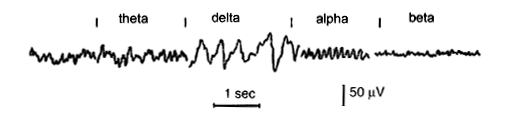
\includegraphics[width=\textwidth]{images/EEGrhythms.png}
\caption{EEG rhythms and amplitudes}
\label{fig:EEGrhythms}
\end{figure}



\subsection{Skin temperature}
\label{subsec:setup:phys-signals:temp}

Since the human skin forms the interface between the human body and
the thermal environment, skin temperature describes heat
transfer. Thermocouples, thermistors, and infrared sensors are the
thermally sensitive components generally applied for this
purpose \cite{van2006evaluation}.


\subsection{Sweating}
\label{subsec:setup:phys-signals:eda}

The human skin displays several forms of bioelectric phenomena,
especially in areas of the extremities such as the fingers, palms of
the hands, and soles of the feet \cite{PoligraphLesson}. The terms
galvanic skin resistance (GSR) and electrodermal activity (EDA) refer
to the electrical properties of the skin.


The physiological basis of the GSR and the EDA is a change in
autonomic tone occurring in the skin in response to a change in the
state of the subject. Changes in peripheral autonomic tone alter
sweating and cutaneous blood flow \cite{PoligraphLesson}. These
disturbances can be quantified by applying an electrical potential
between two points of skin contact and measuring the resulting current
flow between them \cite{braithwaite2013guide}. This way GSR and EDA
signals are formed. The principal components of the latter are shown
in \figref{EDAcomponents}

\begin{figure}[!ht]
\centering
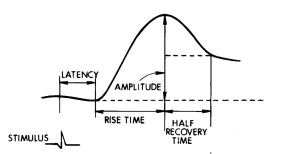
\includegraphics[width=0.7\textwidth]{images/EDAcomponents.png}
\caption{Principal EDA components}
\label{fig:EDAcomponents}
\end{figure}
